\ylDisplay{Vedru} % Ülesande nimi
{Mihkel Kree} % Autor
{lõppvoor} % Voor
{2015} % Aasta
{G 8} % Ülesande nr.
{9} % Raskustase
{
% Teema: Dünaamika
\ifStatement
Kasti sees on vedru külge riputatud koormis. Nii kast kui koormis on massiga $m$. Vedru mass on tühiselt väike ning selle jäikustegur on $k$. Kastil lastakse kõrguselt $h$ vabalt maha kukkuda nii, et langemise ajal on koormis tasakaaluolekus. Kokkupõrkel pehme pinnaga jääb kast hetkeliselt paigale. Kast on piisavalt kõrge selleks, et koormis vastu kasti ei põrkaks. Vedrut ei suruta ühelgi hetkel täielikult kokku.\\
\osa Milline on vähim kõrgus $h_\text{m}$, millelt kukkudes hüppab kast tagasi üles?\\
\osa Kastil lasti kukkuda punktis a) leitud algkõrguselt $h\approx h_\text{m}$. Kui pika ajavahemiku $t$ veedab kast maapinnal enne üles kerkimist? 

\emph{Märkus.} Pange tähele, et vabalangemises olev koormis on kaaluta olekus ning seetõttu on vedru langemise ajal välja venitamata. Maapinnale jõudes pole koormis enam tasakaaluasendis ning hakkab seetõttu uue tasakaaluasendi ümber võnkuma nurksagedusega $\omega =\sqrt{\frac{k}{m}}$.
\fi


\ifHint
Vastu maapinda kukkudes jääb kast hetkeliselt paigale ning koormis hakkab võnkuma ümber uue tasakaaluasendi ehk ümber punkti, kus vedru pinge tasakaalustab koormisele mõjuva raskusjõu. Järgneva liikumise käigus on kõige kriitilisem punkt see, kus koormis on kõige kõrgemas punktis. Sellisel juhul on kastile mõjuva vedru jõud maksimaalne.
\fi


\ifSolution
\osa Hetkeks, mil kast maapinnale jõuab, on koormis omandanud kiiruse $v_i=\sqrt{2gh}$. Seejärel hakkab vedru võnkuma ümber uue tasakaaluasendi ehk ümber punkti, kus vedru pinge tasakaalustab koormisele mõjuva raskusjõu: $ky_0=mg$. Tasakaaluasendisse jõudmiseks peab koormis veel täiendavalt läbima kauguse $y_0=\frac{mg}{k}$. Olgu vedru võnkumise amplituud $A$. Kõige ülemises punktis jääb koormis hetkeks seisma ning kokkusurutud vedru avaldab nii koormisele kui kastile jõudu $k(A-y_0)$. Kast hüppab üles tingimusel $mg = k(A-y_0)$, millest 
\[
A = \frac{mg}{k}+y_0 =2y_0.
\]
Rakendame nüüd energia jäävust. Võnkumise ülemises punktis on kineetiline energia muutunud gravitatsiooni ja vedru potentsiaalseks energiaks. 
\[
mgh=\frac{mv_i^2}{2} = mg(A-y_0) + \frac{1}{2}k(A-y_0)^2 = \left(1+ \frac{1}{2}\right)mgy_0 = \frac{3}{2}mgy_0,
\]
millest saame otsitavaks kõrguseks
\[
h_\text{min} = \frac{3}{2}y_0 = \frac{3mg}{2k} = \frac{3g}{2\omega^2}.
\]
\begin{center}
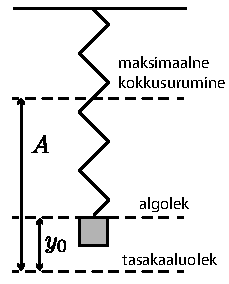
\includegraphics[width=0.35\textwidth]{2015-v3g-08-vedruJoonis_v2.pdf}
\end{center}
\osa Teisele küsimusele vastates lähtume harmoonilise võnkumise omadustest. Veendume esmalt, et konstantse jõu $mg$ lisamine nihutab tasakaaluasendit, kuid jätab võnkumist kirjeldava võrrandi samaks. Tõepoolest, lugedes koordinaadi $y$ alguspunktiks uue tasakaaluasendi, on meie vedru võnkumine kirjeldatav võrrandiga
\[
ma = m \ddot{y} = -k(y-y_0) - mg = -ky.
\]
Sellise võnkumise nurksagedus on muidugi $\omega=\sqrt{k/m}$ ning periood $T=\frac{2\pi}{\omega}$. Kui hakkaksime aega lugema hetkest, mil koormis läbib tasakaaluasendit, siis kuluks vedru maksimaalselt kokku surumiseks kolm veerandperioodi ($\frac{3}{4}T$: kast liigub alla, tagasi tasakaaluasendisse ja üles), sest langemiskõrguse $h=h_\text{min}$ korral saab kast hüpata vaid koormise kõige ülemises asendis. Paraku ei alusta me aja arvestamist mitte tasakaaluasendist, vaid hetkest, mil vedru on välja venitamata. Peame seega arvesse võtma lisaaega $\Delta t$, mis kulub koormisel vahemaa $y_0$ läbimiseks. Kuna koormis ei liigu konstantse kiirendusega, siis seos $s=at^2/2$ siin ei kehti. $\Delta t$ leidmiseks lähtume harmoonilise võnkumise faasist $\varphi$, mis kulub algasendist tasakaaluasendisse jõudmiseks. Seda faasi on lihtne avaldada koordinaatide abil, pidades silmas, et amplituud $A$ vastab koordinaadi faasinihkele $\pi/2$ tasakaaluasendi suhtes. Nimelt $y_0=A\sin\varphi$, millest
\[
\varphi = \arcsin(y_0/A) = \arcsin(1/2) = \frac{\pi}{6}.
\]
Faasi $\varphi$ läbimiseks kuluv aeg on
\[
\Delta t = \frac{\varphi}{\omega}=\frac{1}{12}T.
\]
Järelikult veedab kast maapinnal kuni üles kerkimiseni aja
\[
t = \frac{3}{4}T + \Delta t = \frac{5}{6}T = \frac{5\pi}{3\omega}.
\]
\fi


\ifEngStatement
% Problem name: Spring
In a box there is a weight fixed to a spring. Both the box and the weight have a mass $m$. The mass of the spring is insignificantly small and its stiffness is $k$. The box is dropped down freely from a height $h$ so that during the falling the weight is in an equilibrium state. Colliding with a soft surface the box stays still for a moment. The box is high enough for the weight not to collide against the box. Not for one moment is the spring completely pressed together.\\
\osa What is the smallest dropping height $h_\text{m}$ for the box to jump back up again?\\
\osa The box was dropped from a height $h\approx h_\text{m}$ found in the section a). For what time $t$ will the box be on the ground before starting to rise up?\\
\emph{Note.} Notice that during a free fall the mass inside the box is in a weightless state and because of that the spring is not stretched out during the fall. When reaching the ground the weight is not in the equilibrium position anymore and because of that starts to swing around a new equilibrium position with an angular frequency of $\omega =\sqrt{\frac{k}{m}}$.
\fi


\ifEngHint
Falling against the surface the box will stay still for a moment and the weight starts to oscillate around the new equilibrium position, in other words around the point where the spring’s tension balances the gravity force applied to the weight. During the consequent motion the most critical point is where the weight is at the highest point. In this case spring’s force applied to the box is maximal.
\fi


\ifEngSolution
a) By the moment when the box reaches the ground the weight has reached velocity a $v_i=\sqrt{2gh}$. Next the spring starts to oscillate around a new equilibrium position, meaning around the point where the spring’s tension balances gravity force applied to the weight: $ky_0=mg$. To reach the equilibrium position the weight has to additionally cover a distance $y_0=\frac{mg}{k}$. Let the amplitude of the spring’s oscillation be $A$. At the highest point the weight stays still for a moment and the spring that is pressed together applies the force $k(A-y_0)$ to both the weight and the box. The box jumps up in the condition $mg = k(A-y_0)$, where $A = \frac{mg}{k}+y_0 =2y_0$. Let us now use the conservation of energy. At the upper point of the oscillation the kinetic energy has changed into the potential energy of gravitation and the spring. $mgh=\frac{mv_i^2}{2} = mg(A-y_0) + \frac{1}{2}k(A-y_0)^2 = \left(1+ \frac{1}{2}\right)mgy_0 = \frac{3}{2}mgy_0$ where we get the desired height $h_\text{min} = \frac{3}{2}y_0 = \frac{3mg}{2k} = \frac{3g}{2\omega^2}$.
\begin{center}
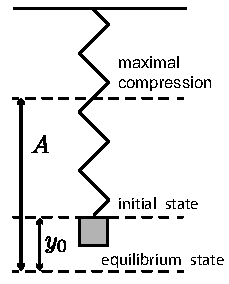
\includegraphics[width=0.35\textwidth]{2015-v3g-08-vedruJoonis_v2_ing}
\end{center}
b) To answer the second question we follow the characteristics of harmonic oscillation. First let us make sure that the addition of constant force $mg$ shifts the equilibrium position but lets the equation describing the oscillation stay the same. Indeed, choosing the new equilibrium position to be the $y$ coordinate’s origin our spring’s oscillation is described by the formula $ma = m \ddot{y} = -k(y-y_0) - mg = -ky$. The angular frequency of this oscillation is $\omega=\sqrt{k/m}$ and period $T=\frac{2\pi}{\omega}$. If we started to count the time from the moment where the weight goes through the equilibrium position then it would take maximally three quarter periods to press the spring together ($\frac{3}{4}T$: the box moves down, back to the equilibrium position and up) because in the case where the falling height is $h=h_\text{min}$ the box can only jump in the case of the uppermost position of the weight. Unfortunately we do not begin to count the time from the equilibrium position but from the moment where the spring is not stretched out. Thus, we have to consider the additional time $\Delta t$ that it takes the weight to cover the distance $y_0$. Because the weight does not move with a constant velocity then the relation $s=at^2/2$ does not apply here. To find $\Delta t$ we use the oscillation phase $\varphi$ of the harmonic oscillation that it takes to reach the equilibrium position from the initial position. This phase can be easily expressed with the help of coordinates while remembering that the amplitude $A$ corresponds to the phase shift $\pi/2$ with respect to the equilibrium position. Namely $y_0=A\sin\varphi$ where $\varphi = \arcsin(y_0/A) = \arcsin(1/2) = \frac{\pi}{6}$. The time it takes to cover the phase $\varphi$ is $\Delta t = \frac{\varphi}{\omega}=\frac{1}{12}T$. Therefore the box stays on the ground for the time $t = \frac{3}{4}T + \Delta t = \frac{5}{6}T = \frac{5\pi}{3\omega}$ before rising up.
\fi
}